\documentclass[a4paper, 10pt, oneside]{memoir}
\usepackage{style}

\usepackage{animate}
\usepackage{wrapfig}
\usepackage{import}

% ТИТУЛЬНИК
\title{
\vspace{4cm}
\normalfont \normalsize 
\horrule{0.5pt} \\[0.4cm]
\huge Конспект по обучению с подкреплением
\horrule{2pt} \\[0.5cm]
}

\author{Издание дописывающееся и дорабатывающееся}

\date{\normalsize\today}

\begin{document}
% Делаем мат. формулы жирными! 
\mathversion{bold}

% Вставляем титульник
\maketitle
\thispagestyle{empty}

% Роботы
\begin{center}
    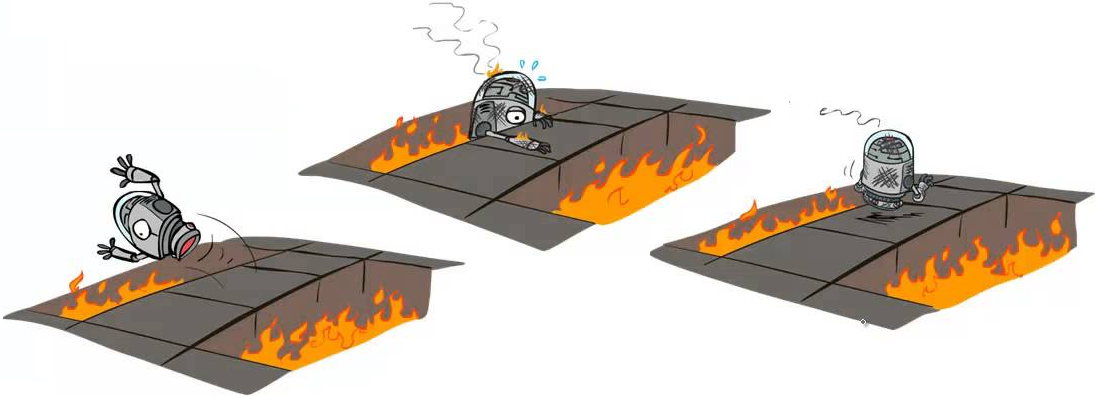
\includegraphics[width=0.7\textwidth]{Images/robot.png}
\end{center}

% Дисклеймер
\vspace{2cm}
\begin{center}
\textcolor{ChadBlue}{\underline{\textbf{Дисклеймер}}}

\vspace{1cm}
Work in Progress
\end{center}

% В файле собрано моё понимание теории по обучению с подкреплением. Предпринята отчаянная попытка как-то унифицировать ход рассуждений, обозначения и определения, а также соблюсти тонкий баланс между строгостью и понятностью изложения. Из-за этого в тексте и в доказательствах потенциально присутствует откровенная лажа; \textbf{соответственно, просьба всем в обязательном порядке собирать все опечатки, баги, вероятные ошибки, несогласованные обозначения и WTF-моменты} и отправлять в любом виде мне (например, маркером в акробате пометить).

% Вставляем оглавление
\newpage
\tableofcontents*

% Поехали!
\import{1.Setup/}{1. Chapter.tex}
\import{2.MetaHeuristics/}{2. Chapter.tex}
\import{3.ClassicTheory/}{3. Chapter.tex}
\import{4.ValueBased/}{4. Chapter.tex}
\import{5.PolicyGradient/}{5. Chapter.tex}

% \vspace{2cm}
% \begin{center}
% That's all, folks!
% \end{center}

\newpage

\appendix

\chapter{Приложение}

\import{Appendix/}{NaturalGradient.tex}
\import{Appendix/}{QLearningConvergence.tex}

%END PAGE-----------------------------------------------
\import{}{sources.tex}

% \newpage
% \thispagestyle{empty}
% \begin{center}
% \vspace*{12cm}
% 
\includegraphics[width=10cm]{Images/reach.jpg}
% \end{center}
\end{document}